\documentclass{article}

\usepackage{fancyhdr}
\usepackage{extramarks}
\usepackage{amsmath}
\usepackage{amsthm}
\usepackage{amsfonts}

% TikZ/Graphics
\usepackage{tikz}
\usetikzlibrary{
    automata,  % for markov chains
    arrows.meta,  % arrow tips (technically deprecated)
    backgrounds,  % background layers
    decorations,  % decorations applied to paths
    decorations.markings,  % additional markings on paths
    decorations.pathmorphing,  % deforming decorations
    decorations.pathreplacing,  % replacing paths
    calligraphy,  % for calligraphic brace (must be loaded after decorations)
    patterns,  % patterns for filling areas
    positioning,  % better custom positioning
    shapes,  % various shapes
    intersections,
}
\usepackage{forest}
\usepackage{circuitikz}
\usepackage{pgfplots}
\pgfplotsset{compat=1.18}
\usepgfplotslibrary{
    groupplots,  % grouping pgf plots
}

\usepackage[plain]{algorithm}
\usepackage{algpseudocode}
\usepackage{hyperref}
\usepackage{multicol}
\usepackage{mathrsfs}
\usepackage{pifont}
\usepackage{circledsteps}

\usetikzlibrary{automata,positioning}

%
% Basic Document Settings
%

\topmargin=-0.45in
\evensidemargin=0in
\oddsidemargin=0in
\textwidth=6.5in
\textheight=9.0in
\headsep=0.25in

\linespread{1.1}

\pagestyle{fancy}
\lhead{\hmwkAuthorName}
\chead{\hmwkClass\ (\hmwkClassInstructor): \hmwkTitle}
\rhead{\firstxmark}
\lfoot{\lastxmark}
\cfoot{\thepage}

\renewcommand\headrulewidth{0.4pt}
\renewcommand\footrulewidth{0.4pt}

\setlength\parindent{0pt}

%
% Create Problem Sections
%

\newcommand{\enterProblemHeader}[1]{
    \nobreak\extramarks{}{Problem \arabic{#1} continued on next page\ldots}\nobreak{}
    \nobreak\extramarks{Problem \arabic{#1} }{Problem \arabic{#1} continued on next page\ldots}\nobreak{}
}

\newcommand{\exitProblemHeader}[1]{
    \nobreak\extramarks{Problem \arabic{#1} }{Problem \arabic{#1} continued on next page\ldots}\nobreak{}
    \stepcounter{#1}
    \nobreak\extramarks{Problem \arabic{#1}}{}\nobreak{}
}

\setcounter{secnumdepth}{0}
\newcounter{partCounter}
\newcounter{homeworkProblemCounter}
\setcounter{homeworkProblemCounter}{1}
\nobreak\extramarks{Problem \arabic{homeworkProblemCounter}}{}\nobreak{}

%
% Homework Problem Environment
%
% This environment takes an optional argument. When given, it will adjust the
% problem counter. This is useful for when the problems given for your
% assignment aren't sequential. See the last 3 problems of this template for an
% example.
%
\newenvironment{homeworkProblem}[2][-1]{
    \ifnum#1>0
        \setcounter{homeworkProblemCounter}{#1}
    \fi
    \section{Problem \arabic{homeworkProblemCounter}: #2}
    \setcounter{partCounter}{1}
    \enterProblemHeader{homeworkProblemCounter}
}{
    \exitProblemHeader{homeworkProblemCounter}
}

%
% Homework Details
%   - Title
%   - Due date
%   - Class
%   - Section/Time
%   - Instructor
%   - Author
%

\newcommand{\hmwkTitle}{Homework\ \#3}
\newcommand{\hmwkDueDate}{February 15, 2025}
\newcommand{\hmwkClass}{Discrete Mathematics}
\newcommand{\hmwkClassTime}{Section A}
\newcommand{\hmwkClassInstructor}{Professor Satish Rao}
\newcommand{\hmwkAuthorName}{\textbf{Zachary Brandt}}
\newcommand{\hmwkAuthorEmail}{\href{mailto:zbrandt@berkeley.edu}{zbrandt@berkeley.edu}}

%
% Title Page
%

\title{
    \vspace{2in}
    \textmd{\textbf{\hmwkClass:\ \hmwkTitle}}\\
    \normalsize\vspace{0.1in}\small{Due\ on\ \hmwkDueDate\ at 4:00pm}\\
    \vspace{0.1in}\large{\textit{\hmwkClassInstructor}}
    \vspace{3in}
}

\author{\hmwkAuthorName \\ \hmwkAuthorEmail}
\date{}

\renewcommand{\part}[1]{\textbf{\large Part \Alph{partCounter}}\stepcounter{partCounter}\\}

%
% Various Helper Commands
%

% Useful for algorithms
\newcommand{\alg}[1]{\textsc{\bfseries \footnotesize #1}}

% For derivatives
\newcommand{\deriv}[1]{\frac{\mathrm{d}}{\mathrm{d}x} (#1)}

% For partial derivatives
\newcommand{\pderiv}[2]{\frac{\partial}{\partial #1} (#2)}

% Integral dx
\newcommand{\dx}{\mathrm{d}x}

% Alias for the Solution section header
\newcommand{\solution}{\textbf{\large Solution}}

% Probability commands: Expectation, Variance, Covariance, Bias
\newcommand{\E}{\mathrm{E}}
\newcommand{\Var}{\mathrm{Var}}
\newcommand{\Cov}{\mathrm{Cov}}
\newcommand{\Bias}{\mathrm{Bias}}

\begin{document}

\maketitle

\pagebreak

\begin{homeworkProblem}{Edge Colorings}

    An edge coloring of a graph is an assignment of colors to edges in a graph where any two edges incident to the same vertex have different colors. An example is shown on the left.

    \begin{center}
        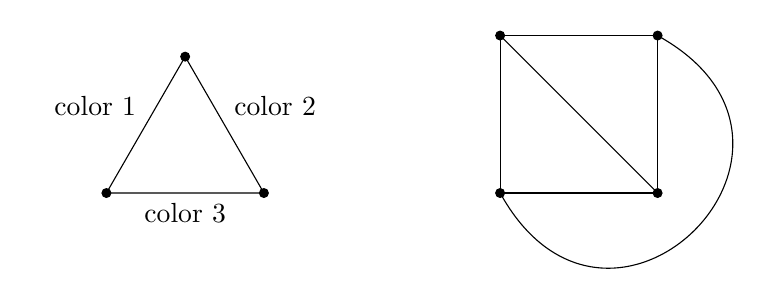
\begin{tikzpicture}
            \clip (-1, -1) rectangle (8, 2.1);
    
            \node[circ] (n1) at (0, 0) {};
            \node[circ] (n2) at (1, {sqrt(3)}) {};
            \node[circ] (n3) at (2, 0) {};
            \draw (n1) -- node[above left] {color 1} (n2)
            -- node[above right] {color 2} (n3)
            -- node[below] {color 3} (n1);
    
            \node[circ] (m1) at (5, 0) {};
            \node[circ] (m2) at (5, 2) {};
            \node[circ] (m3) at (7, 2) {};
            \node[circ] (m4) at (7, 0) {};
            \draw (m1) -- (m2) -- (m3) -- (m4) -- (m1);
            \draw (m2) -- (m4);
            \draw (m1) edge[out=-60, in=-30, looseness=2.5] (m3);
        \end{tikzpicture}
    \end{center}

    \begin{itemize}
        \item[A)] (You may use the numbers $1,2,3$ for colors. A figure is shown on the right.)
        \item[B)] Prove that any graph with maximum degree $d \geq 1$ can be edge colored with $2d-1$ colors. 
        \item[C)] Prove that a tree can be edge colored with $d$ colors where $d$ is the maximum degree of any vertex.
    \end{itemize}
    
\end{homeworkProblem}

\pagebreak

\begin{homeworkProblem}{Touring Hypercube}

    An the lecture, you have seen that if $G$ is a hypercube of dimension $n$, then
    \begin{itemize}
        \item The vertices of $G$ are the binary strings of length $n$.
        \item $u$ and $v$ are connected by an edge if they differ in exactly one bit location.
    \end{itemize}
    
    A \emph{Hamiltonian tour} of a graph (with $n \geq 2$ vertices) is a tour that visits every vertex exactly once.

    \begin{itemize}
        \item[A)] Prove that a hypercube has an Eulerian tour if and only if $n$ is even.
        \item[B)] Prove that every hypercube has a Hamiltonian tour. 
    \end{itemize}
    
\end{homeworkProblem}

\pagebreak

\begin{homeworkProblem}{Planarity and Graph Complements}

    Let $G = (V, E)$ be an undirected graph.  We define the complement of $G$ as $\overline{G} = (V, \overline{E})$ where $\overline{E} = \{(i,j) \mid i,j \in V, i \neq j\} - E$; that is, $\overline{G}$ has the same set of vertices as $G$, but an edge $e$ exists is $\overline{G}$ if and only if it does not exist in $G$.

    \begin{itemize}
        \item[A)] Suppose $G$ has $v$ vertices and $e$ edges.  How many edges does $\overline{G}$ have?
        \item[B)] Prove that for any graph with at least 13 vertices, $G$ being planar implies that $\overline{G}$ is non-planar.
        \item[C)] Now consider the converse of the previous part, i.e., for any graph $G$ with at least 13 vertices, if $\overline{G}$ is non-planar, then $G$ is planar. Construct a counterexample to show that the converse does not hold.
    \end{itemize}

    \textit{Hint: Recall that if a graph contains a copy of $K_5$, then it is non-planar. Can this fact be used to construct a counterexample?}
        
\end{homeworkProblem}

\pagebreak

\begin{homeworkProblem}{Modular Practice}

    Solve the following modular arithmetic equations for $x$ and $y$. For each subpart, show your work and justify your answers.

    \begin{itemize}
        \item[A)] $9x+5 \equiv 7 \pmod{13}$.
        \item[B)] Prove that $3x+12 \equiv 4 \pmod{21}$ does not have a solution.
        \item[C)] The system of simultaneous equations $5x+4y \equiv 0 \pmod{7}$ and $2x+y \equiv 4 \pmod{7}$. 
        \item[D)] $13^{2023} \equiv x \pmod{12}$.
        \item[E)] $7^{62} \equiv x \pmod{11}$.
    \end{itemize}
    
\end{homeworkProblem}

\pagebreak

\begin{homeworkProblem}{Wilson's Theorem}

    Wilson's Theorem states the following is true if and only if $p$ is prime:
    \[(p - 1)! \equiv -1 \pmod{p}.\]
    Prove both directions (it holds if AND only if $p$ is prime).

    Hint for the if direction: Consider rearranging the terms in $(p - 1)! = 1 \cdot 2 \cdot \cdots \cdot (p - 1)$ to pair up terms with their inverses, when possible. What terms are left unpaired?

    Hint for the only if direction: If $p$ is composite, then it has some prime factor $q$.  What can we say about $(p-1)! \pmod{q}$?
    
\end{homeworkProblem}

\pagebreak

\begin{homeworkProblem}{How Many Solutions?}
    Consider the equation $ax \equiv b \pmod p$ for prime $p$. In the below three
    parts, when we discuss solutions, we mean a solution $x$ in the range $\{0, 
    1, \dots p-1\}$. In addition, include justification for your answers to all
    the subparts of this problem.

    \begin{itemize}
        \item[A)] For how many pairs $(a,b)$ does the equation have a unique solution?
        
        When $a \equiv 0 \pmod{p}$, for any $x$, the equation will have the same
        solution where $ax \equiv 0 \equiv b \pmod{p}$. Therefore, for the equation
        to produce a unique solution for $x$, $a \not\equiv 0 \pmod{p}$. There are 
        then $p-1$ options for $a$ and $p$ options for $b$ to form pairs, i.e.,
        there are $p(p-1)$ pairs $(a,b)$ for which the equation has unique solutions.
        
        \item[B)] For how many pairs $(a,b)$ does the equation have no solution?
        
        The equation has no solutions when $a \equiv 0 \pmod{p}$ but $b \not\equiv
        0 \pmod{p}$. Therefore, there is one option for $a$, 0, and $p-1$ not zero
        options for $b$, i.e., there are $p-1$ pairs $(a, b)$ for which the equation
        has no solutions. 

        \item[C)] For how many pairs $(a,b)$ does the equation have $p$ solutions?
        
        When both $a$ and $b$ are equivalent to 0 modulos $p$, there aren't any 
        unique solutions but there are $p$ solutions, since all elements in the 
        set $\{0, 1, \dots p-1\}$ times 0 will be equivalent to 0 modulos $p$.
        There is one pair, $(0, 0)$, for which the equation has $p$ solutions. 

    \end{itemize}

    Now, consider the equation $ax \equiv b \pmod{pq}$ for distinct primes $p,q$.
    In the below three parts, when we discuss solutions, we mean a solution $x$ 
    in the range $\{0, 1, \dots pq-1\}$.

    \begin{itemize}
        \item[D)] If $\gcd(a, pq) = p$, show that there exists a solution if and 
        only if $b = 0 \pmod p$. 

        If $b \equiv 0 \pmod{p}$, then $b \equiv 0 \pmod{pq}$ as well. In which 
        case $ax \equiv b \equiv 0 \pmod{pq}$ has a solution when $x = 0$. 

        If we only know that there exists a solution, we need to show that $b
        \equiv 0 \pmod{p}$. Since $a$ and $pq$ share $p$ as a greatest common 
        divisor, $b$ must also be a multiple of $p$ for $ax \equiv b \pmod{pq}$ 
        to hold. Therefore, $b \equiv 0 \pmod{p}$.


        \item[E)] If $\gcd(a, pq) = p$ and there is a solution $x$, show that there
        are exactly $p$ solutions. (Hint: consider how you can generate another solution
        $x + \_\_\_$)

        % From part D), it must then be the case, as per the biconditional, that $b$
        % is equivalent to 0 modulos $p$. Therefore, the equation $ax \equiv b \pmod{pq}$
        % becomes
        % \[
        %     \begin{split}
        %         ax \equiv b & \pmod{pq} \\
        %         k \cdot px \equiv l \cdot p & \pmod{pq} \\
        %         kx \equiv l & \pmod{pq}
        %     \end{split}
        % \]
        % Since both left- and right-hand sides of the equivalency became multiples 
        % of $p$, dividing by $p$ considers the equivalencies modulos $q$. 
        We can express $a$ as a multiple $k$ of $p$ in our equation to answer
        the question
        \[
            \begin{split}
                ax \equiv b & \pmod{pq} \\
                kp \cdot x \equiv b & \pmod{pq} \\
            \end{split} 
        \]

        To generate $x + \_\_\_$ solutions, we can add multiples $l$ of $q$ to 
        $x$, e.g. $kp(x + 2q)$, as each $klpq$ is equivalent to 0 modulos $q$. 
        We can only add up to the $p$ multiple of $q$ however, at which point 
        the solutions cycle and are identical to earlier ones.  

        \item[F)] For how many pairs $(a,b)$ are there exactly $p$ solutions? 
        
        The requirements from the last part are that $a$ and $pq$ share a greatest 
        common divisor of $p$, and form part D) that $b \equiv 0 \pmod{p}$. $b$
        can be expressed as a multiple of $p$, e.g. $kp$. $k$ must be less than
        $q$, otherwise $b$ becomes equivalent to $pq$ or out of range. Therefore,
        there are $q$ values $b$ can take on where $k \in \{ 0, 1, \dots, q-1 \}$.
        Similarly for $a$, it can be expressed as a multiple of $p$, e.g. $mp$.
        For $a$ to be divisible by $p$, but also not have $pq$ as a greatest
        common divisor and stay in the range, $m$ must be in the set $\{ 1, 2, \dots, q-1 \}$.
        Therefore, there are $q \cdot (q-1)$ pairs with exactly $p$ solutions.


    \end{itemize}
    
\end{homeworkProblem}

\end{document}